% Exemple de fichier fonctionnnant avec la classe CAp2012.cls
% Base :  
%	Classe pf2010.cls adpatée de pf2003 par Jean CHarlet
%	Classe pf2003.cls adpatée de ic2001 par Jean CHarlet
%
% 	Classe ic2001.cls adpatée de EEGDRI3 par Jean CHarlet
%
% 	Classe EEGDRI3.cls adpatée de ic2000 par Jean CHarlet
%
% 	Classe IC'2000 (ic2000.cls) par Jean Charlet
%
% 	adaptée de la classe IC'99 (afia99.cls) développée par Fabien Torre

%\documentclass{CAp2012}
\documentclass[publibook-draft]{CAp2012}

\newcommand{\verbfichex}{CAp2012.\xspace}
\newcommand{\verbfichclass}{CAp2012.cls\xspace}
\newcommand{\verbfichbst}{CAp2012.bst\xspace}


%\usepackage[pdftex]{pstricks}

\usepackage{verbatim}
\usepackage{subfigure}
\usepackage[french]{babel}
\usepackage[utf8]{inputenc}
\usepackage[T1]{fontenc}
\usepackage{amsmath}
\usepackage{amssymb}

\usepackage{natbib}
\usepackage{algorithm}
\usepackage{algorithmic}
%%% francisation des algorithmes
\renewcommand{\algorithmicrequire} {\textbf{\textsc{Entrées:}}}
\renewcommand{\algorithmicensure}  {\textbf{\textsc{Sorties:}}}
\renewcommand{\algorithmicwhile}   {\textbf{tantque}}
\renewcommand{\algorithmicdo}      {\textbf{faire}}
\renewcommand{\algorithmicendwhile}{\textbf{fin tantque}}
\renewcommand{\algorithmicend}     {\textbf{fin}}
\renewcommand{\algorithmicif}      {\textbf{si}}
\renewcommand{\algorithmicendif}   {\textbf{finsi}}
\renewcommand{\algorithmicelse}    {\textbf{sinon}}
\renewcommand{\algorithmicthen}    {\textbf{alors}}
\renewcommand{\algorithmicfor}     {\textbf{pour}}
\renewcommand{\algorithmicforall}  {\textbf{pour tout}}
\renewcommand{\algorithmicdo}      {\textbf{faire}}
\renewcommand{\algorithmicendfor}  {\textbf{fin pour}}
\renewcommand{\algorithmicloop}    {\textbf{boucler}}
\renewcommand{\algorithmicendloop} {\textbf{fin boucle}}
\renewcommand{\algorithmicrepeat}  {\textbf{répéter}}
\renewcommand{\algorithmicuntil}   {\textbf{jusqu'à}}

\floatname{algorithm}{Algorithme}


%\newtheorem{algorithm}{Algorithme}
\newtheorem{definition}{Définition}

%%%%%%%%%%%%%%%%%%%%%%%%%%%%%%%%%%%%%%%%%%%%%%%%%%%%%%%%%%%%%%%%%%%%%%%
% Titre court si le titre fait plus de 40 caractères
%%%%%%%%%%%%%%%%%%%%%%%%%%%%%%%%%%%%%%%%%%%%%%%%%%%%%%%%%%%%%%%%%%%%%%%

\shorttitle{Batch Inverse Reinforcement Learning}

\shortouvrage{CAp 2012}

% Titre, auteur, pas de date

\title{Batch Imitation via Inverse Reinforcement Learning Without Solving the Direct Problem}

\author{\fontsize{12}{12}\selectfont{Edouard Klein\inst{1}\inst{2}, Matthieu Geist\inst{1}, Olivier Pietquin\inst{1}\inst{3}}}

\institute{
Sup\'elec,\\
IMS Research group, France\\
\texttt{prenom.nom@supelec.fr}
\and
Equipe ABC,\\
LORIA-CNRS, France
\and
UMI 2958\\
GeorgiaTech-CNRS, France
}


\begin{document}
\maketitle


\begin{abstract}
  Cette contribution traite du problème de l'apprentissage par imitation par le biais de l'apprentissage par renforcement inverse ({\it Inverse Reinforcement Learning, IRL}). Dans ce contexte, un expert accomplit une tâche qu'un agent doit essayer de reproduire. L'IRL part du postulat que l'expert optimise avec succès une fonction d'utilité et cherche à deviner cette fonction (appelée récompense) avec pour entrée une trace du comportement de l'expert. Les algorithmes d'IRL existants nécessitent une ou plusieurs des conditions suivantes pour fonctionner : trajectoires complètes de la part de l'expert, un modèle génératif pour les estimations de type Monte-Carlo, la connaissance des probabilités de transition, la capacité de résoudre le problème direct (celui du {\it Reinforcement Learning, RL}) de manière répétée et l'accès à la strategie complète de l'expert. Notre contribution consiste en un nouvel algorithme d'IRL levant toutes ces contraintes. En utilisant une méthode supervisée dans laquelle nous introduisons implicitement la structure du processus décisionnel de Markov ({\it Markov Decision Process, MDP}) sous-jacent, nous créons un algorithme basé sur une descente de sous gradient et possèdant une faible complexité tant en échantillons que calculatoire.
  \motscles{Apprentissage par renforcement, Apprentissage par renforcement inverse, Processus Decisionnel de Markov}
\end{abstract}
%%%%%
\section{Introduction}
%%%%%
\begin{itemize}
\item Introduction informelle sur les processus de décision séquentiels
\item Intérêt de l'apprentissage par démonstration
\item Intérêt de l'IRL pour faire de l'apprenticeship learning
\item Rapide point sur les limitations des algos d'IRL actuels
\begin{itemize}
\item \cite{ng2000algorithms} : Probabilités de transitions devant être connues
\item \cite{abbeel2004apprenticeship} et toutes les approches résumées dans \cite{neu2009training}: Résolution du problème direct à chaque itération
\end{itemize}
\end{itemize}
%%%%%
\section{Background}
%%%%%
\label{back.sec}
%%%
\subsection{Principe}
%%%
Le cadre dans lequel nous plaçons notre étude est celui de la prise de décisions séquentielle. La configuration du système à contrôler est alors décrite à chaque instant $t$ par un état $s_t \in S$. Confronté à cet état, l'agent doit prendre un décision $a_t\in A$. Le système évolue alors vers l'état suivant $s_{t+1}$ selon une certaine probabilité $p(s_{t+1}|s_t, a_t)$. Une politique de contrôle déterministe \footnote{On peut se restreindre au cas déterministe sans perte de généralité} $\pi : S\rightarrow A$ définit le comportement d'un agent confronté à un tel problème de décision séquentielle.\\

Dans le cadre plus restreint de l'apprentissage par renforcement, pour guider la résolution de ce problème il faut fournir à l'agent une fonction de récompense $R : S \rightarrow \mathbb{R}$ qui lui apprendra le degré auquel l'état dans lequel il se trouve est désirable. Une des forces de l'apprentissage par renforcement réside dans le fait que l'agent ne va pas apprendre à maximiser la récompense immédiate mais au contraire un critère prenant le futur en compte. On définit pour ce faire la fonction de valeur $V^\pi$ :
\begin{eqnarray}
\label{Vdef.eqn}
V^\pi(s) &=& E\left[\left.\sum_t\gamma^tR(s_t)\right|s_0=s,\pi\right]\\
&=& R(s) + \gamma\sum_{s'}p(s'|s,\pi(s))V^\pi(s')
\end{eqnarray}
où $\gamma$ est un facteur d'actualisation strictement plus petit que $1$. Une politique optimale est alors définie comme une politique dont la fonction de valeur $V^*$ (appelée fonction de valeur optimale) vérifie :
\begin{equation}
\forall \pi, \forall s, V^*(s) \geq V^\pi(s).
\end{equation}
L'ensemble formé par l'espace d'état $S$, l'espace d'action $A$, les probabilités de transition $p$, le facteur $\gamma$ et la fonction de récompense $R$ forme un processus décisionnel de Markov ({\it Markov Decision Process, MDP}).\\

Parfois, définir la fonction de récompense est une tâche ardue alors qu'il est possible à l'opérateur de convenablement contrôler le système de manière intuitive. Un exemple de ce type de tâche est la conduite d'une voiture. Nous accompplissons ce genre de choses au quotidien sans trop y penser mais nous serions bien en peine de préciser les poids précis que nous attribuons aux différents critères tels que la distance nous séparant de la voiture devant nous, la brutalité avec laquelle nous appuyons sur la pédale de frein lorsqu'un danger se présente et ainsi de suite. Dans de tels cas, il est utile d'inférer la récompense à partir d'un comportement démontré.\\

C'est la définition de l'apprentissage par renforcement inverse. Le problème est de retrouver la fonction de récompense optimisée par un expert. Usuellement l'expert est considéré comme un agent optimal dans un MDP et l'on a accès ou bien à la politique complète $\pi_E$ de l'expert ou bien à quelques trajectoires tirées selon cette politique.\\

Ce problème est mal posé dans la mesure où étant donné un comportement, il n'y a pas unicité de la récompense pour lequel ce comportement est optimal. Particulièrement, la récompense uniformément nulle remplit ce critère dans la mesure où tout comportement est optimal vis à vis de cette récompense.
%%%
\subsection{Considérations techniques}
%%%
La recherche de la politique optimale en apprentissage par renforcement se fait souvent en utilisant une fonction voisine de la fonction de valeur, la fonction de qualité définie par :
\begin{eqnarray}
Q^\pi(s,a) &=& E\left[\left.\sum_t\gamma^tR(s_t)\right|s_0=s,a_0=a,\pi\right]\\
&=& R(s) + \gamma\sum_{s'}p(s'|s,a)V^\pi(s').
\end{eqnarray}
La politique optimale se définit simplement à partir de la fonction de qualité optimale $Q^*$ via un mécanisme glouton :
\begin{equation}
\pi^*(s) \in \arg\max_a Q^*(s,a).
\end{equation}
Dès lors, l'approximation de la fonction de valeur (terme qui employé au sens large désigne aussi la fonction de qualité) est un thème central en apprentissage par renforcement. Une caractéristique répandue dans la litérature est l'utilisation d'un cadre d'approximation linéaire où, après avoir défini des attributs vectoriels $\phi: S\times A \rightarrow \mathbb{R}^k$, l'on va chercher un vecteur de paramètres $\omega$ tel que l'on ait une bonne approximation de la fonction de qualité :
\begin{equation}
\hat Q (s,a) = \omega^T\phi(s,a)\approx Q(s,a).
\end{equation}
Il est naturel d'adopter le même type d'approche pour l'apprentissage par renforcement inverse, c'est à dire de considérer que l'inconnue du problème, la récompense $R$, peut être bien approximée grâce à un vecteur de poids $\theta$ et des attributs vectoriels $\psi : S\rightarrow \mathbb{R}^p$ :
\begin{equation}
\hat R(s) = \theta^T\psi(s)\approx R(s).
\end{equation}

Introduire cette expression dans la définition de la fonction de valeur (Equation \ref{Vdef.eqn}) fait apparaître un terme intéressant et dont l'usage est assez répandu dans les algorithmes existants :
\begin{eqnarray}
V^\pi(s) &=& E\left[\left.\sum_t\gamma^t\theta^T\psi(s_t)\right|s_0=s,\pi\right]\\
V^\pi(s) &=& \theta^TE\left[\left.\sum_t\gamma^t\psi(s_t)\right|s_0=s,\pi\right]\\
V^\pi(s) &=& \theta^T\mu^\pi(s)
\end{eqnarray}

Le terme $\mu^\pi$ est appelé la {\it feature expectation} d'une politique. Il existe plusieurs variantes basées sur la même définition que nous venons de donner. Dans sa version la plus spécifique, notée simplement $\mu^\pi$, il s'agit en toute rigueur de l'expression :
\begin{eqnarray}
\mu^\pi = E\left[\left.\sum_t\gamma^t\psi(s_t)\right|s_0\sim d,\pi\right],
\end{eqnarray}
où $d$ est une distribution sur l'état initial. Il peut également être utile de le définir sous la forme $\mu^\pi(s,a)$ où son rôle par rapport à $\mu^\pi(s)$ est le même que celui de $Q$ par rapport à $V$ :
\begin{eqnarray}
\mu^\pi(s,a) = E\left[\left.\sum_t\gamma^t\psi(s_t)\right|s_0=s,a_0=a,\pi\right].
\end{eqnarray}
On peut noter que si deux politiques ont la même {\it feature expectation}, alors ces deux politiques ont la même valeur vis à vis de la récompense, quel que soit le vecteur de poids $\theta$ définissant celle-ci. En effet 
\begin{eqnarray}
\mu^{\pi_1} = \mu^{\pi_2} &\Rightarrow& \theta^T\mu^{\pi_1} = \theta^T\mu^{\pi_2}\\
& \Rightarrow& V^{\pi_1} = V^{\pi_2}.
\end{eqnarray}
La {\it feature expectation} de l'expert, $\mu_E$, pouvant être calculée sans forcément avoir accès à l'intégralité de la politique $\pi_E$, certains algorithmes de la litérature ont, comme nous allons le voir, pour objectif de minimiser la distance entre les {\it feature expectations} respectives de l'agent et de l'expert, afin d'obtenir un agent dont le comportement à la même valeur que celui de l'expert.
%%%%%
\section{Loss-augmented Feature Expectation Matching}
%%%%%
%%%
\subsection{Principe}
%%%
Notre algorithme cherche à minimiser la fonction de risque suivante :
\begin{equation}
  R_N(q) = {1\over N} \sum_{i=1}^N\left(\max_{a}(q(s_i,a) + l(s_i,a)) - q(s_i,a_i) \right)
\end{equation}
Dans le travail de \citep{ratliff2007imitation}, cette fonction de risque est introduite pour décrire un classifieur utilisant la fonction de score $q$ et qui à un élément $s$ associe la label $a = \arg\max\limits_a q(s,a)$. Cela est très similaire à l'équation
  \begin{equation}
  \label{greedy.eqn}
  \pi^*(s) = \arg\max_{a} Q^*(s,a)
  \end{equation}
  qui décrit le mécanisme glouton liant fonction de valeur optimale et politique optimale. La politique de l'expert étant une politique optimale, elle doit respecter cette équation. Minimiser notre fonction de risque revient donc à chercher une fonction $q$ compatible avec la fonction de valeur optimale de l'expert. En effet, considérons que la fonction de perte $l$ est uniformément nulle et regardons ce qui se passe lorsque la fonction de risque $R_N(q)$ est minimisée. On introduit $a^* = \arg\max\limits_a(q(s_i,a))$. Si la fonction de risque $R_N(q)$ est positive, alors il arrive pour certains $i$ que $q(s_i,a^*) > q(s_i,a_i)$. Cela signifie que la fonction $q$ ne permet pas de justifier le choix de l'expert. A l'opposé, si l'on parvient à anuller $R_N(q)$, on a $\forall i, q(s_i,a^*) = q(s_i,a_i)$, et donc $a_i \in \arg\max\limits_a q(s_i,a)$, ce qui justifie le choix de l'expert.\\

   La fonction de perte $l$ permet d'introduire de la connaissance à priori en laissant l'opérateur influer sur la forme de la fonction $q$ recherchée.\\

   Nous allons profiter de la structure présente dans $Q$ pour introduire la notion de \emph{feature expectation} dans le problème. On rappelle qu'en IRL il est classique d'écrire $Q(s,a) = \theta^T \mu(s,a)$. Nous nous basons donc sur la \emph{feature expectation} de l'expert, $\mu_E$ et un vecteur de paramètres $\theta$ contrôlant la fonction de récompense que l'on recherche pour réécrire la fonction de risque que nous allons minimiser :
  \begin{equation}
   R_N(\theta) = {1\over N} \sum_{i=1}^N\left(\max_{a}(\theta ^T \mu_E(s_i,a) + l(s_i,a)) - \theta ^T \mu_E(s_i,a_i) \right)
   \end{equation}
   Il faut noter ici l'utilisation non pas de $\mu_E : S\rightarrow \mathbb{R}^p$ mais de $\mu_E : S\times A \rightarrow \mathbb{R}^k$. Cette dernière partage avec la première la même relation que $Q$ partage avec $V$, c'est à dire que l'on dispose d'un degré de liberté en plus correspondant à la prochaine action, qui peut différer de celle choisie par l'expert.

   
   De la même manière que précedemment, on note $a^* = \arg\max\limits_{a} = \theta_t ^T \mu_E(s_i,a) + l(s_i,a)$, l'expression de la fonction de risque devient alors :
   \begin{eqnarray}
   R_N(\theta) &=& {1\over N} \sum_{i=1}^N\left(\theta ^T \mu_E(s_i,a^*) + l(s_i,a^*) - \theta ^T \mu_E(s_i,a_i) \right)\\
   &=& {1\over N} \sum_{i=1}^N\left(\theta^T\left(\mu_E(s_i,a^*) - \mu_E(s_i,a_i)\right) + l(s_i,a^*)  \right).
   \end{eqnarray}

   La présence d'un $\max$ dans cette expression (caché dans le $a^*$) nous oblige à utiliser le sous gradient dont la règle est que le sous gradient du $\max$ est le gradient de l'$\arg\max$.

   Le sous gradient de cette expression est donc : 
   \begin{equation}
   \nabla L_N(\theta) =  {1\over N}\sum_{i=1}^N\left(\mu_E(s_i,a^*) - \mu_E(s_i,a_i)\right).
   \end{equation}

   Une descente de gradient sur le risque donne la règle d'update suivante :
   \begin{equation}
   \theta_{t+1} = \theta_t -\alpha_t{1\over N}\sum_{i=1}^N\left(\mu_E(s_i,a^*) - \mu_E(s_i,a_i)\right),
   \end{equation}

   avec $\alpha_t$ un pas d'apprentissage. L'algorithme complet est détaillé algorithme \ref{LAFEM.alg}.

\begin{algorithm}
\caption{LAFEM ({\it Loss-Augmented Feature Expectation Matching})}
\label{LAFEM.alg}
\begin{algorithmic}
  \REQUIRE une fonction de perte $l : S\times A \rightarrow \mathbb R$
  \REQUIRE la \emph{feature expectation} de l'expert $\mu_E : S\times A \rightarrow \mathbb R ^p$
  \REQUIRE un pas d'apprentissage $\alpha : \mathbb N \rightarrow \mathbb R$
  \REQUIRE des données provenant de l'expert $\{(s_i,a_i)\}_{i=1..N}$
  \REQUIRE un vecteur de paramètres initial $\theta_0$
  \REQUIRE un nombre maximum d'itérations $T\in \mathbb N$
  \REQUIRE une description de l'espace d'action $A$

     
  \FOR {T iterations}
  \STATE $\Delta\theta \leftarrow [0...0]^T$
    \FORALL{ $(s_i,a_i)$}
    \STATE $a^* \leftarrow \arg\max\limits_{a} = \theta_t ^T \mu_E(s_i,a) + l(s_i,a)$
    \STATE $\Delta\theta \leftarrow \Delta\theta + \mu_E(s_i,a^*) - \mu_E(s_i,a_i)$
    \ENDFOR
    \STATE $\theta_{t+1} = \theta_t -\alpha_t{1\over N}\Delta\theta$
    \ENDFOR
    \RETURN $\theta_T$
\end{algorithmic}
\end{algorithm}
%%%%%
\section{Résultats expérimentaux}
%%%%%
%%%
\subsection{Calcul de $\mu_E$}
%%%
L'algorithme présenté repose sur le calcul de la {\it feature expectation} de l'expert, $\mu_E$. Selon les informations dont on dispose, plusieurs méthodes peuvent être utilisées pour la calculer.

La définition du vecteur $\mu_E$ étant proche de celle de la fonction de valeur, en adaptant les algorithmes de programmation dynamique destinés au calcul de la fonction de valeur on obtient une règle de la forme :
\begin{equation}
\mathbf \mu^\pi = \mathbf\Phi + \gamma P_\pi\mathbf\mu^\pi
\end{equation}
permettant le calcul exact de la fonction de valeur pour peu que l'on dispose des probabilités de transitions.\\

Dans le cas plus probable où celles-ci sont inconnues, on peut si l'on dispose d'un simulateur utiliser une simple approximation de Monte-Carlo où pour approximer $\mu_E(s,a) = E\left.\left[\sum\limits_{t=0}^\infty \gamma^t \phi(s)\right|s_0 = s, a_0 = a, \pi_E\right]$ l'on utilise 
\begin{equation}
\hat\mu_E(s,a) = {1\over N}\sum\limits_{i=1}^{N}\sum\limits_{t}\gamma^t\phi(s), s_0=s, a_0=a, a_{t>0} = \pi_E(s_t).
\end{equation}

Finalement si l'on ne dispose ni des probabilités de transition ni d'un simulateur, alors il est possible d'utiliser LSTD$\mu$ (\citep{klein2011batch}), un algorithme permettant l'estimation en {\it batch} de la {\it feature expectation} de l'expert.
%%%
\subsection{Description de la tâche}
%%%
Le problème du pendule inversé à maintenir en équilibre vertical un pendule à un degré de liberté. il s'agit d'un problème classique en apprentissage par renforcement ({\it Reinforcement Learning, RL}). Pour jouer le rôle de notre expert, nous utilisons d'ailleurs la politique trouvée par LSPI, un algorithme de RL décrit par \citet{lagoudakis2003least}. Les différents réglages utilisés, de la valeur de la masse du pendule codée dans notre simulateur jusqu'au choix des fonctions de bases $\phi : S\times A \rightarrow \mathbb{R}^k$ et $\psi : \S \rightarrow \mathbb{R}^p$ sont conformes à ce qui est donné dans cette publication.\\

La politique ainsi trouvée parvient systématiquement à maintenir le pendule en équlibre durant 3000 pas de temps. Ces derniers ayant une valeur d'un dixième de seconde, cela signifie que nous interrompons l'expert après 5 minutes de contrôle sans chute du pendule.\\

Le but de cette expérience est de montrer que notre algorithme est capable, à partir des seuls transitions fournies par l'expert et de la définition des fonctions de bases, de retrouver une récompense telle qu'un agent entraîné sur cette récompense puisse lui aussi faire balancer le pendule durant 5 minutes sans échec. Cela n'est pas trivial étant donné que l'espace d'état est continu et que les données fournies par l'expert n'en couvrent qu'une petite partie (correspondant à la position verticale). Ce dernier point est d'ailleur la raison pour laquelle l'algorithme d'\citet{abbeel2004apprenticeship} ne parvient pas à résoudre le problème à l'aide des seules transitions de l'expert.\\

En effet, comme cela a été montré dans \citep{klein2011batch}, à moins de fournir quelques transitions aléatoires couvrant tout l'espace d'état il est impossible d'utiliser les algorithmes itératifs du type de celui d'\citet{abbeel2004apprenticeship} car ceux-ci requièrent la résolution du problème direct à chaque itération ; résolution qui ne peut se faire si l'on ne dispose que de données ne couvrant qu'une petite partie de l'espace d'état. Comme notre algorithme ne nécessite pas la résolution du problème direct, il ne rencontre pas ce problème.
%%%
\subsection{Illustration des résultats}
%%%
\begin{figure}
  \begin{minipage}[t]{.4\linewidth}
    \begin{center}
       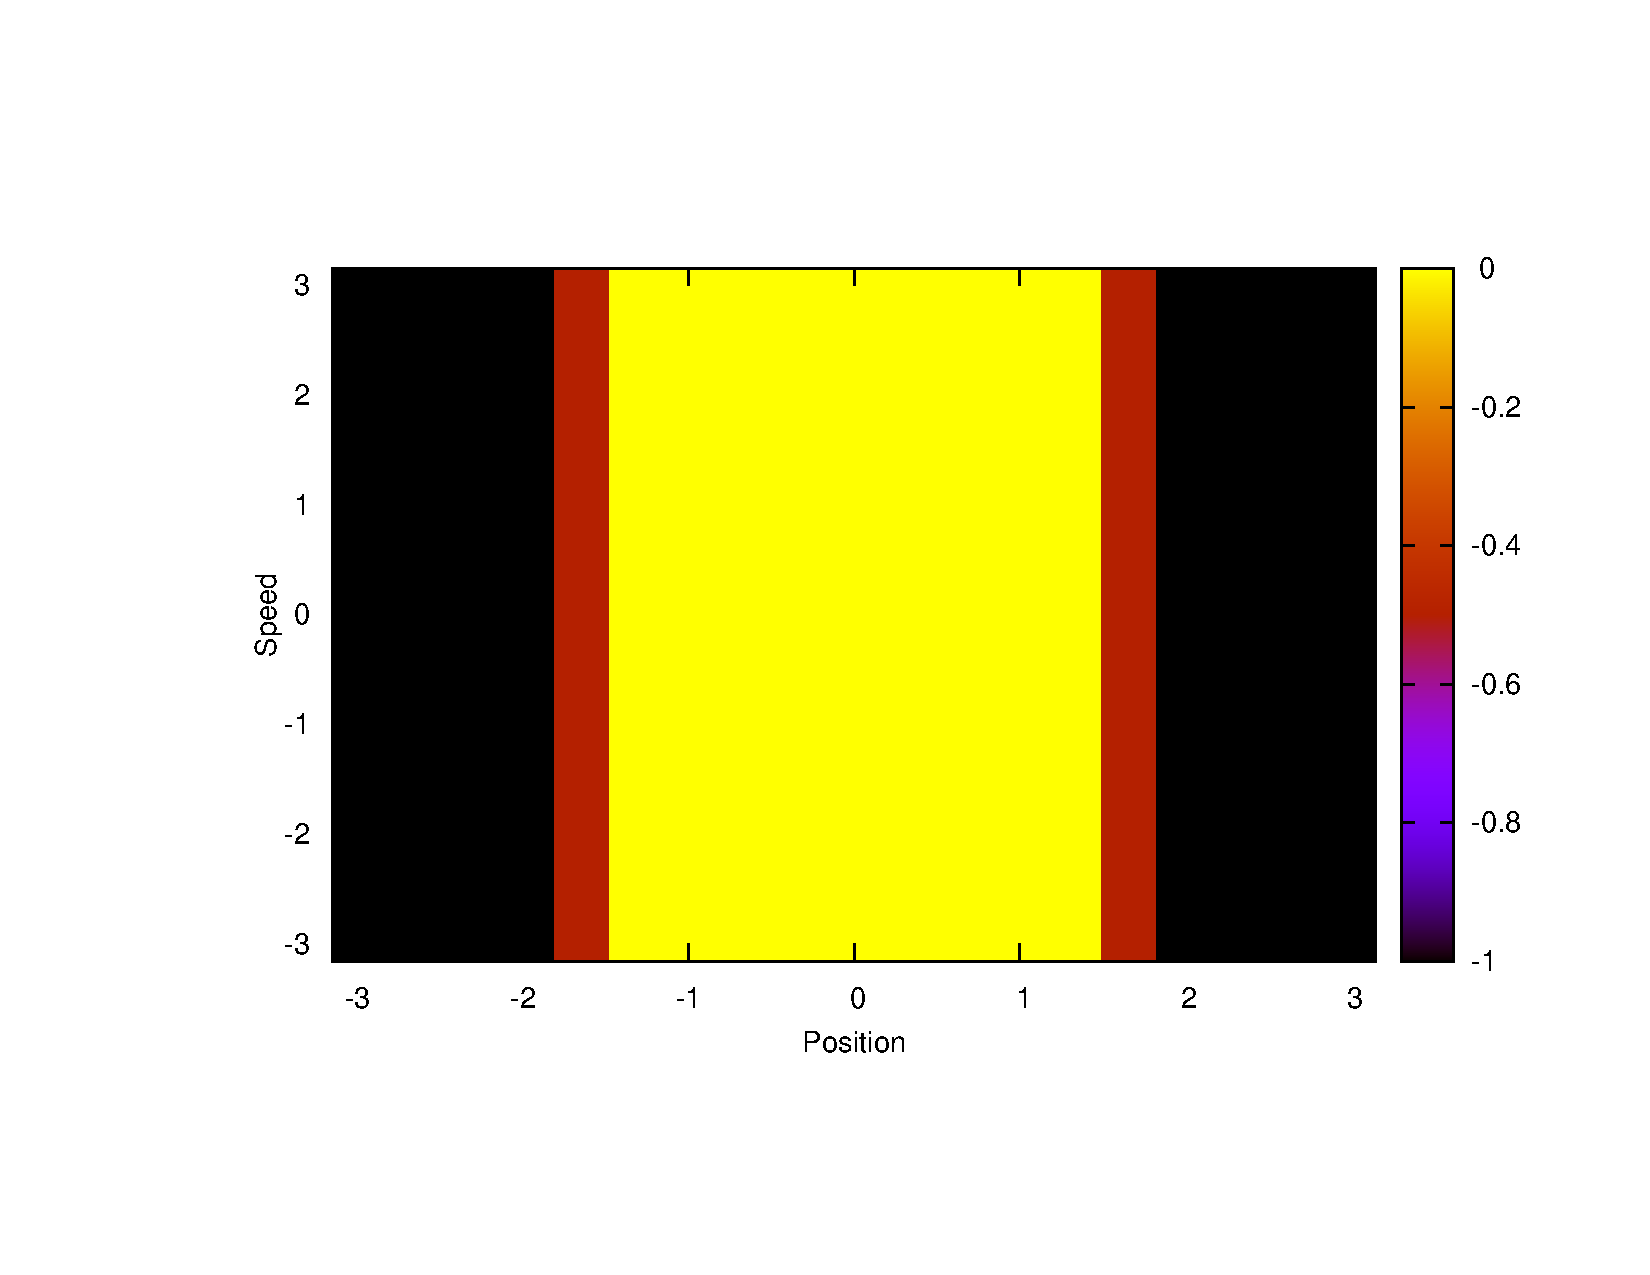
\includegraphics[width=\textwidth]{../InvertedPendulum/LAFEM_Exp3_true_R.pdf}
       \caption{Récompense sur laquelle l'expert a été entraîné}
       \label{trueR.fig}
    \end{center}
\end{minipage}
\hfill
\begin{minipage}[t]{.4\linewidth}
    \begin{center}
       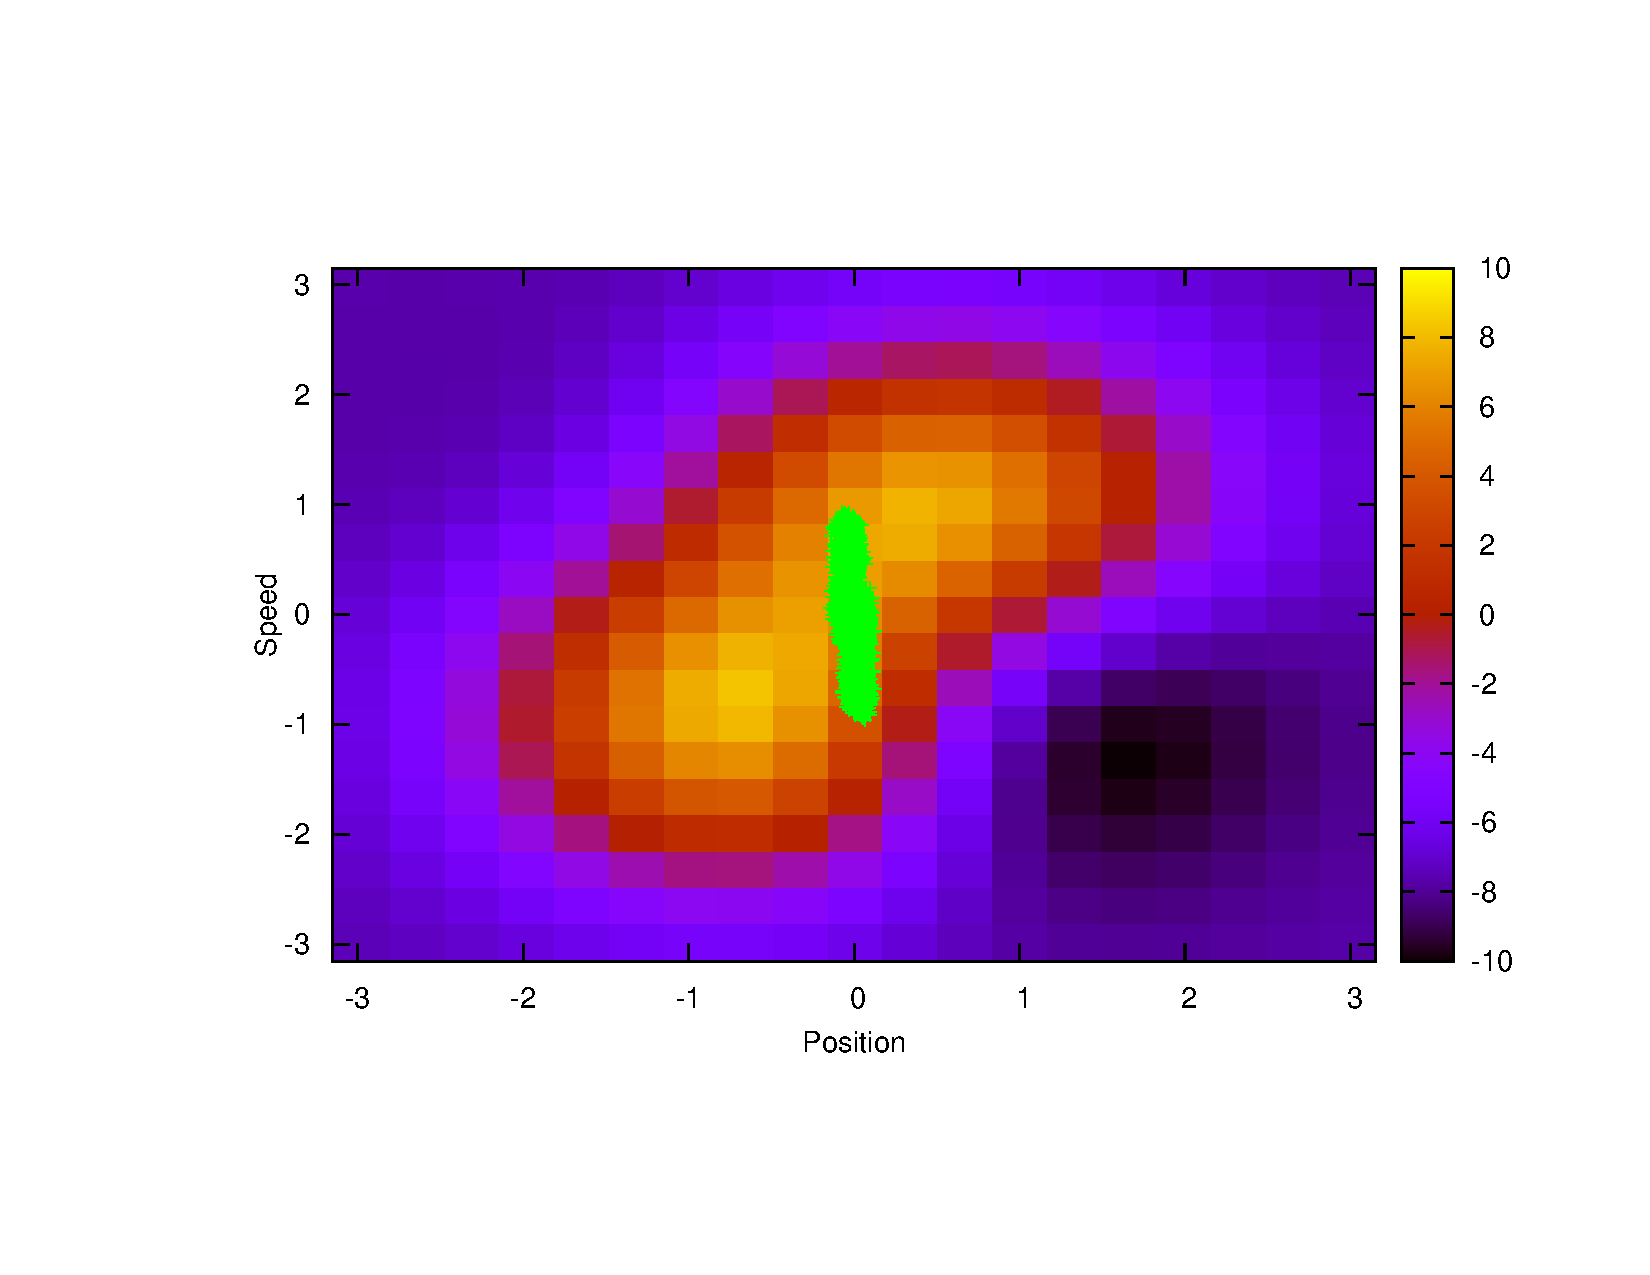
\includegraphics[width=\textwidth]{../InvertedPendulum/LAFEM_Exp3_lafem_R.pdf}
       \caption{Récompense trouvée par LAFEM}
       \label{lafemR.fig}
    \end{center}
\end{minipage}\\
\begin{minipage}[t]{.4\linewidth}
    \begin{center}
       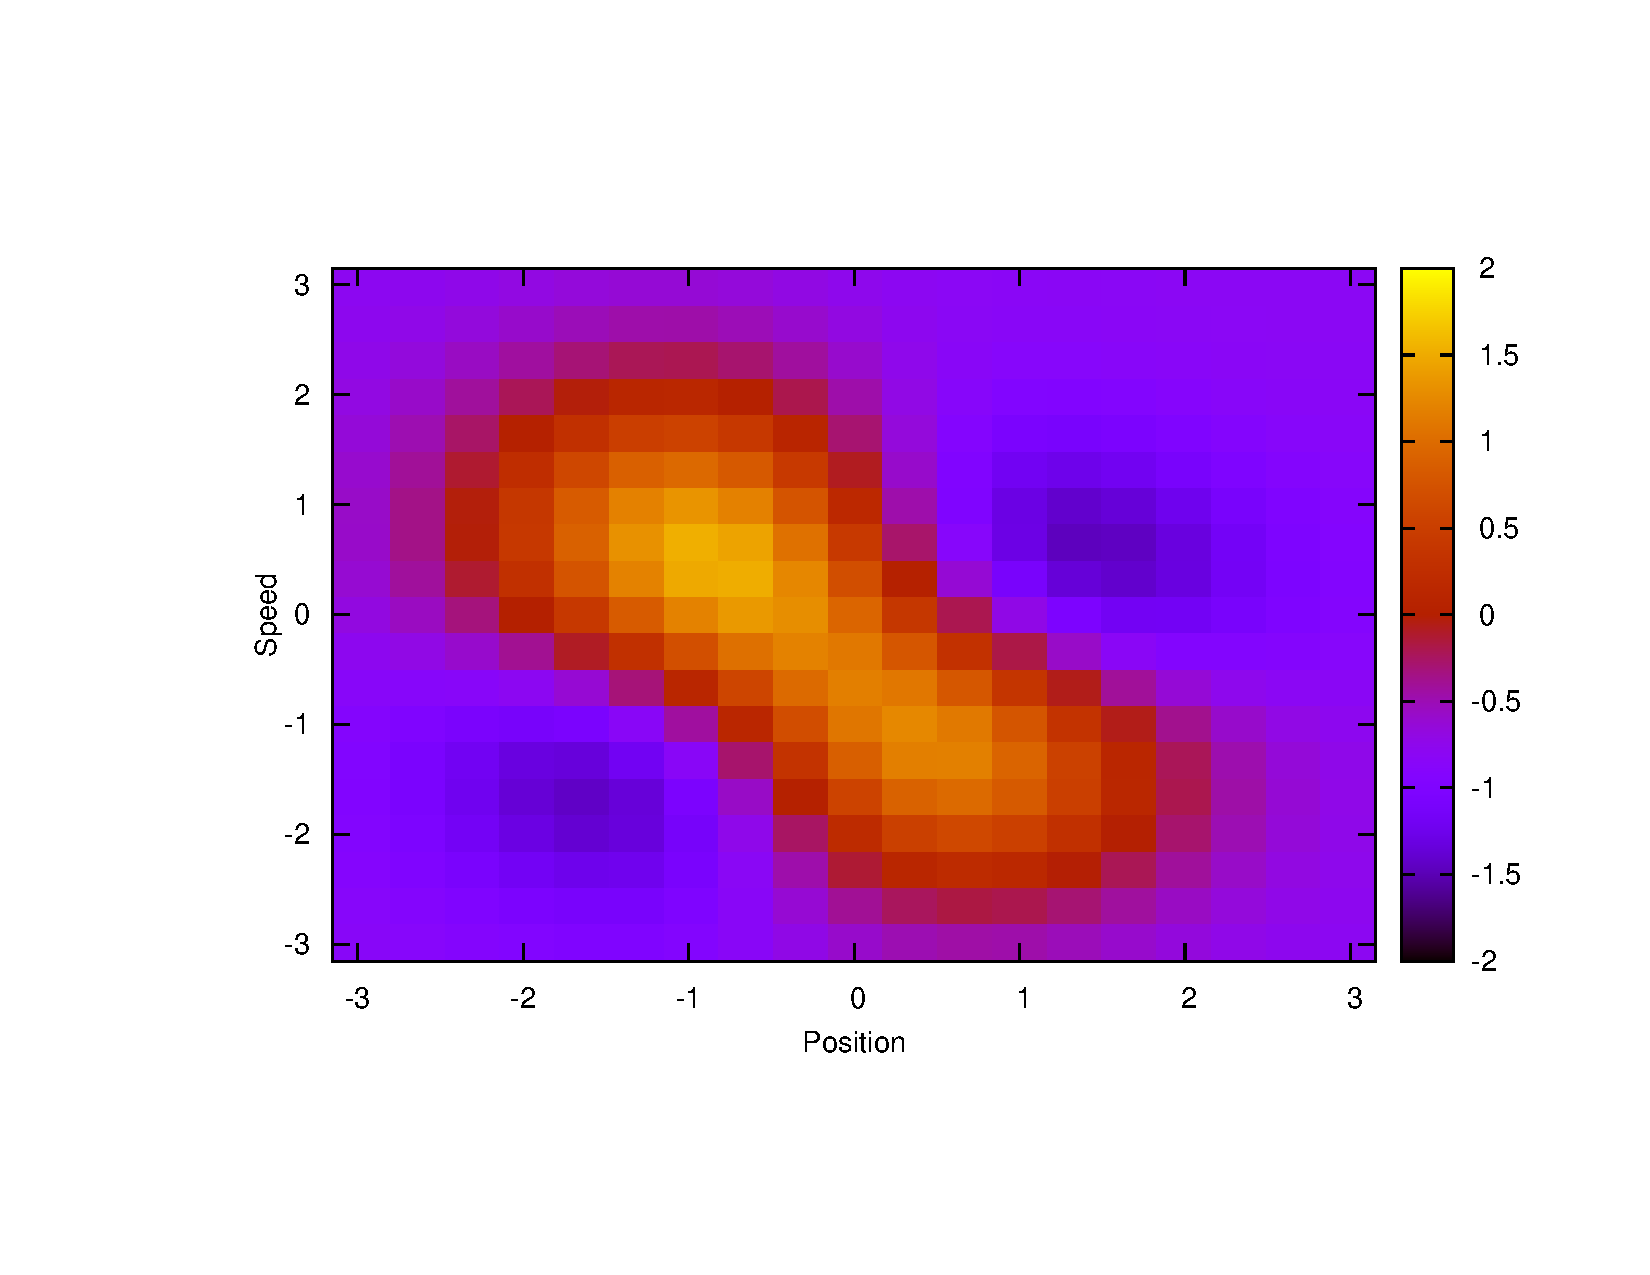
\includegraphics[width=\textwidth]{../InvertedPendulum/LAFEM_Exp3_Vexpert.pdf}
       \caption{Fonction de valeur de l'expert}
       \label{trueV.fig}
    \end{center}
\end{minipage}
\hfill
\begin{minipage}[t]{.4\linewidth}
    \begin{center}
       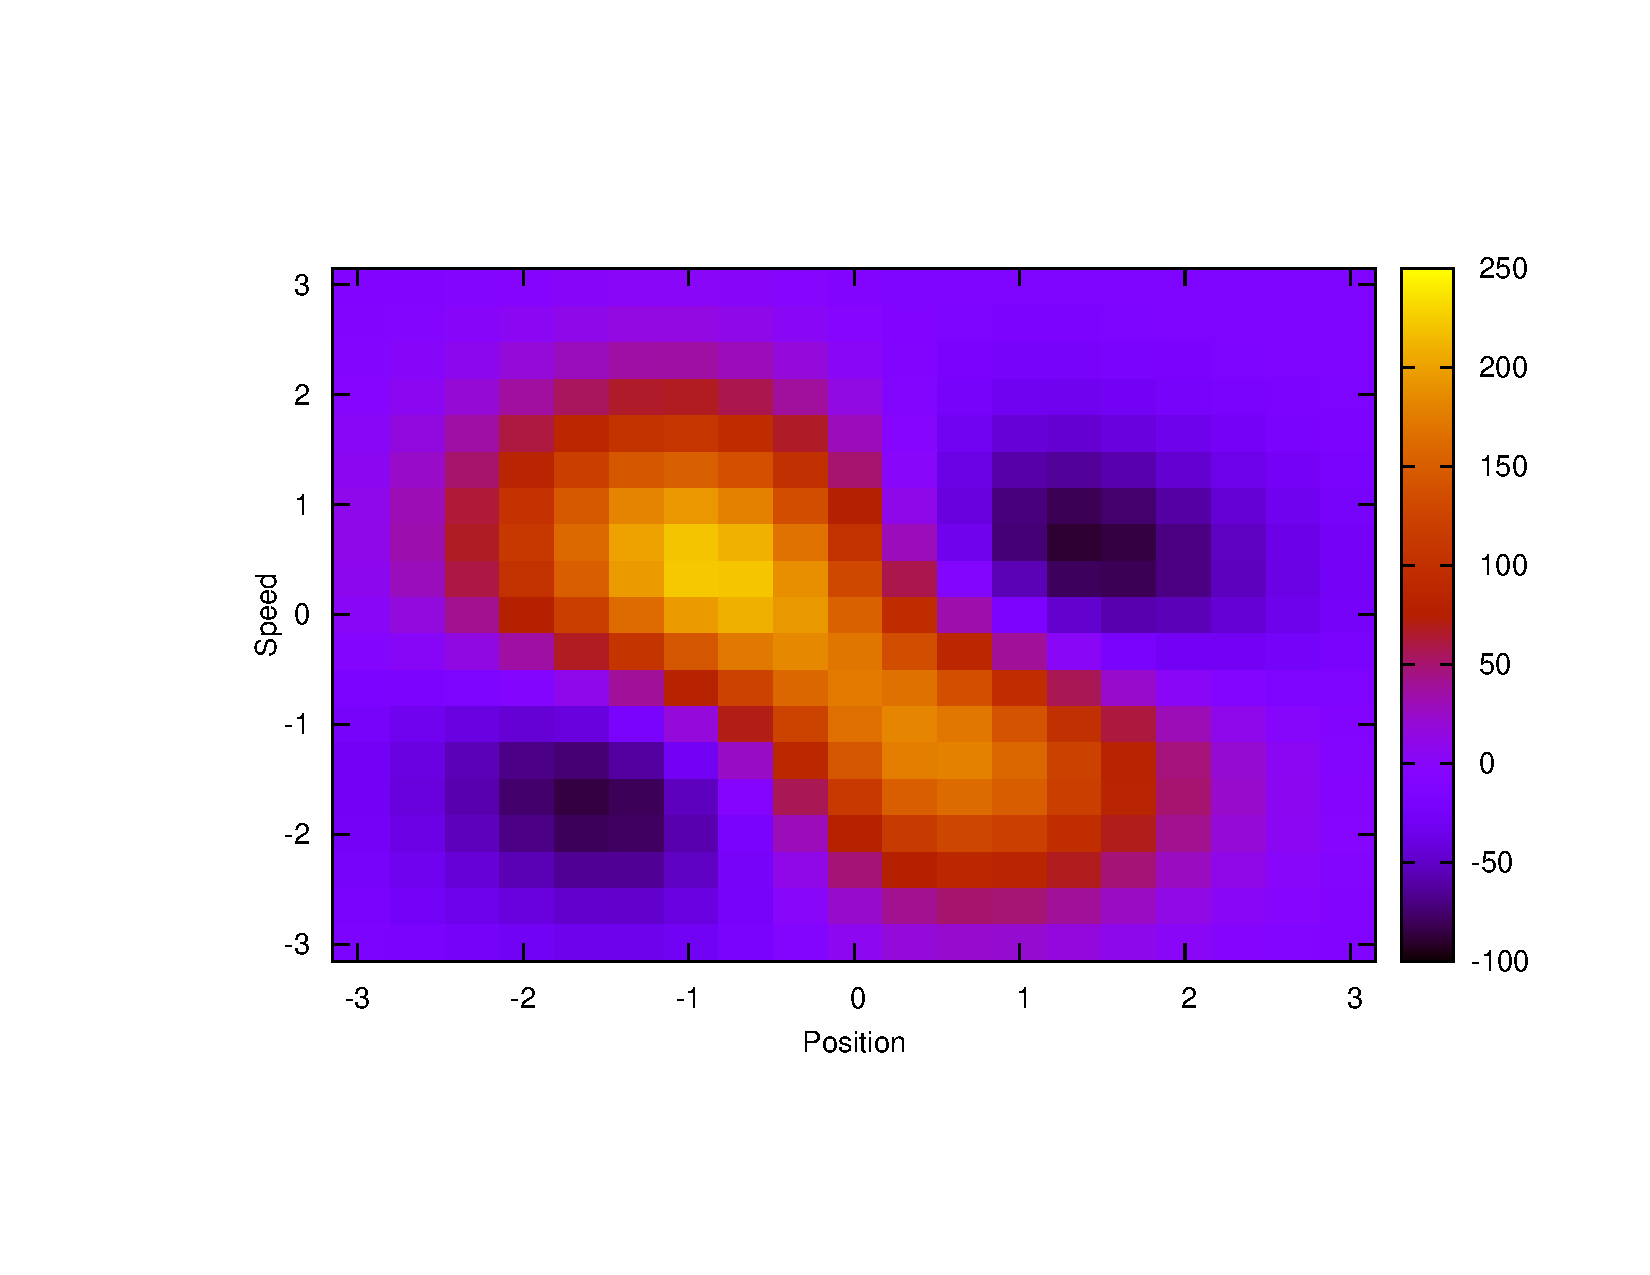
\includegraphics[width=\textwidth]{../InvertedPendulum/LAFEM_Exp3_Vagent.pdf}
       \caption{Fonction de valeur de l'agent entraîné sur la récompense trouvée par LAFEM}
       \label{lafemV.fig}
    \end{center}
\end{minipage}\\
\end{figure}
Afin d'étudier le comportement de notre algorithmes, nous avons établi le protocole expérimental suivant :
\begin{itemize}
 \item Créer une base de données $D_0$ de transitions aléatoires.
 \item Entraîner un expert en utilisant LSPI nourri avec ces transitions ( definissant ainsi $\pi_E : S\rightarrow A$)
 \item Vérifier que l'expert est en mesure de balancer le pendule durant 3000 pas de temps
 \item Créer une base de données $D_E$ de transitions de l'expert, contenant 10 trajectoires de 300 transitions chacune.
 \item Définir $l$ telle que $l(s,a) = 0$ si $a=\pi_E(s)$, $1$ sinon, $l$ est définie sur les états présents dans $D_E$.
 \item Définir $\alpha(t) = 0.1,\forall t$.
 \item Définir $D$ à partir des transitions $D_E$ en enlevant l'état d'arrivée.
 \item Initialiser $\omega_0 = [-1...-1]^T$.
 \item Fixer $T=20$.
 \item Définir $\mu_E(s,a) = E\left.\left[\sum\limits_{t=0}^\infty \gamma^t \phi(s)\right|s_0 = s, a_0 = a, \pi_E\right]$ comme étant en pratique $\hat\mu_E(s,a) =  \omega^T_{\pi_E}\phi(s,a), \omega_{\pi_E} = LSTD\mu(D_E)$.
 \item Faire tourner LAFEM.
 \item Entrainer un agent sur le problème du pendule inversé, avec la récompense trouvée par LAFEM : définir $\pi : S\rightarrow A$.
 \item Vérifier que l'agent parvient lui aussi à maintenir le pendule en équilibre durant 3000 pas de temps.
 \item Afficher la fonction de valeur de l'expert.
 \item Afficher la fonction de valeur de l'agent.
 \item Afficher la fonction de récompense sur laquelle l'expert a été entraîné
 \item Afficher la fonction de récompense retrouvée par LAFEM
\end{itemize}

Si la fonction de récompense trouvée par LAFEM (figure \ref{lafemR.fig}) diffère de celle fournie à l'expert (figure \ref{trueR.fig}) on constate en revanche que les fonctions de valeurs sont très similaires (figures \ref{trueV.fig} et \ref{lafemV.fig}). Cela est une illustration du fait que le problème de l'IRL est mal posé en ceci qu'il n'y a pas qu'une seule récompense pouvant expliquer une politique.\\

Avec le nombre d'échantillons fournis par l'expert (3000 en 10 trajectoires de 300 transitions chacune), l'agent parvient systématiquement à maintenir le pendule en équilibre durant 5 minutes, ce qui est rappelons le notre critère de réussite.

%%%
\subsection{Etude statistique de la qualité de l'imitation}
%%%
Nous souhaitons maintenant empiriquement étudier l'impact de la quantité de données fournies par l'expert sur la qualité du contrôle exhibé par l'agent. Pour cela nous appliquons le protocole suivant :
\begin{itemize}
 \item Créer une base de données $D_0$ de transitions aléatoires.
 \item Entraîner un expert en utilisant LSPI nourri avec ces transitions (ce qui définit $\pi_E : S\rightarrow A$)
 \item Vérifier que l'expert est en mesure de balancer le pendule durant 3000 pas de temps
 \item Créer une base de données $D_E$ de transitions de l'expert. On la crée de 10 trajectoires de 300 transitions chacune.
 \item Définir $l$ telle que $l(s,a) = 0$ si $a=\pi_E(s)$, $1$ sinon, $l$ est définie sur les états présents dans $D_E$.
 \item Définir $\alpha(t) = 0.1,\forall t$ (pifomètre)
 \item Fixer $T=20$ (pifomètre)
 \item Pour différentes quantités de données $N$,
\begin{itemize}
   \item Définir $D_E^N$ en tronquant $D_E$ à ses $N$ premières transitions
   \item Définir $D$ à partir des de $D_E^N$ en enlevant l'état d'arrivée
   \item Définir $\mu_E(s,a) = E\left.\left[\sum\limits_{t=0}^\infty \gamma^t \phi(s)\right|s_0 = s, a_0 = a, \pi_E\right]$ comme étant en pratique $\hat\mu_E(s,a) =  \omega^T_{\pi_E}\phi(s,a), \omega_{\pi_E} = LSTD\mu(D_E^N)$
   \item Initialiser $\omega_0 = [-1...-1]^T$
   \item Faire tourner LAFEM
   \item Entrainer un agent sur le problème du pendule inversé, avec la récompense trouvée par LAFEM : définir $\pi : S\rightarrow A$
   \item Regarder durant combien de pas de temps l'agent arrrive à faire tenir le pendule.
   \item Tracer la courbe donnant la qualité du contrôle (nombre de pas de temps durant lequel l'agent balance le pendule) en fonction de la quantitié de données disponible ($N$)
\end{itemize}
\end{itemize}

Cette expérience a été répétée FIXME:nombre de fois, avec les résultats illutrés FIXME:mettre une figure.
%%%%%
\section{Related Work}
%%%%%
\begin{itemize}
\item Résumé plus détaillé que précédemment des approches IRL actuelles
\item Laïus sur Ratliff et son approche locale (imitation pure) et globale (plain de contraintes)
\end{itemize}
\section{Conclusion and future work}
\begin{itemize}
\item On enlève les contraintes du domaine d'un seul coup, 
\item Il ne reste que la sélection ou détection de features, mais ce n'est pas hors de portée
\item Dans la même veine, il reste la résolution du problème direct une fois la récompense obtenue, il faut peut-être creuser du côté du reward shaping
\item Faible complexité computationnelle
\item Faible complexité en échantillons
\item Il reste des tests à faire sur le Highway driving (Pour ICML ?) et sur des expériences dans la vraie vie (bras robot ?) pour comparer à l'existant
\end{itemize}
%
% Bibliographie
%
\bibliography{Biblio}

\end{document}

